% Chapter Template

\chapter{Design} % Main chapter title

\label{Chapter4} % Change X to a consecutive number; for referencing this chapter elsewhere, use \ref{ChapterX}

%----------------------------------------------------------------------------------------
%	SECTION 1
%----------------------------------------------------------------------------------------

\section{Architecture of the specification}

%-----------------------------------
%	SUBSECTION 1
%-----------------------------------
\subsection{Archictecture diagram}

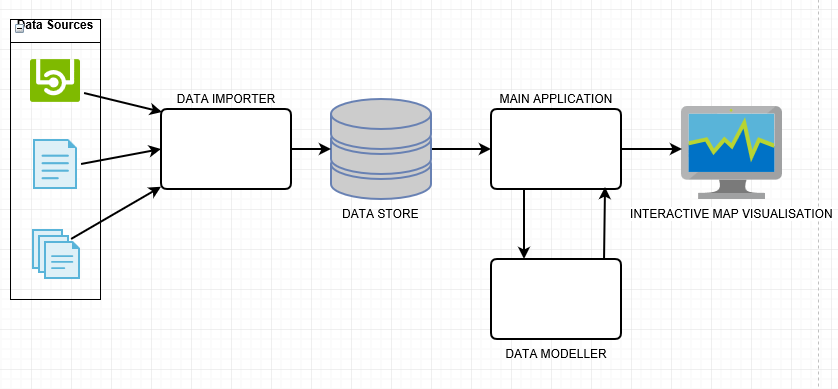
\includegraphics[scale=0.75]{figures/Software_Architecture} % Code example


%-----------------------------------
%	SUBSECTION 2
%-----------------------------------

\subsection{Architecture choices}

For this project two main technologies are being used, Python and Javascript. The majority of the software code has been written in Python, specifically for the data import processes, for the main application which runs the analysis and geocoding and the data modelling component. Python was chosen for these components for a number of factors. Firstly for the data importer, Python has excellent capabilities for data processing allowing the data to be collected and cleaned leveraging the Pandas module. For the main application, Python's geocoding and spatial capabilites were important factors in the choice. The ability to import shape files and reproject coordinate systems leveraging Geopandas and Shapely allowed more flexibility in which datasets were suitable for the project and the option to export to GeoJSON format facilitated the data visualisation.
For the visualisation stages Javascript embedded in a html file was chosen. For this final component of the project Javascript was preferred to Python due to the interactive element required on the map. With the aid of the Leaflet.js package in Javascript I was able to make use of more map features to present any end users with a more complete user experience.


%----------------------------------------------------------------------------------------
%	SECTION 2
%----------------------------------------------------------------------------------------

\section{Components}

The software architecture design for the project has been created with the aim of being able to isolate individual elements in the interest of performance. The system is not dependent on processing a live data feed so it is important that the component that imports the data does not have to run everytime a user would wish to access the interactive map visualisation. The design means that each component can be modified and without affecting the other parts.  


%-----------------------------------
%	SUBSECTION 1
%-----------------------------------
\subsection{Data inputs}
The data input layer is the base layer of the system. This consists of several different types of input including API feeds from the Foursquare platform, csv files collected directly from urls and other data files which have been pre-collected and loaded into the data store. This layer is the most likely to change moving forward as new and updated data sources are published or become available in alternative formats.

%-----------------------------------
%	SUBSECTION 2
%-----------------------------------

\subsection{Data importer}
The data importer software is written in Python and is designed as a series of functions. Each function imports one of the required datasets. Setting these up as seperate functions gives the option to run imports individually. This is an important requirement of the system as certain imports take a considerable amount of time. The iterative nature of the API imports combined with daily rate limits mean that it is only feasible to run the API imports from Foursquare on at most a daily basis. As the system is not reliant on a live feed, the data import software could be run as an overnight batch process. 

%-----------------------------------
%	SUBSECTION 3
%-----------------------------------

\subsection{Data store}
The data store is central to the architecture to safeguard performance levels. As the data imports are best suited to a batch process, the cleaned data files should be stored in the data store for the main application software to run efficiently. The data store is also used for any pre-collected data which cannot be collected directly from a url or API. This imports the data for the 18 base indicators which create the 6 well-being indices.

%-----------------------------------
%	SUBSECTION 4
%-----------------------------------

\subsection{Main application}
The main application software performs a variety of tasks and is written in Python. The first task that the software performs is to take the data that has been imported for the 18 base indicators from the data store. The main application then performs any data manipulation and applies a set of geocoding and spatial functions to standardise the data into a format where everything is aggregated for London Ward geometry. Having standardised, the software then creates the 6 well-being indices using functions drawing on Principal Component Analysis and mean calculation functions which also normalise the data to ensure that each score is between 0 and 100.
These 6 indices are then combined with data showing median house prices and the related quintiles and passed through the regression and classification models chosen through the data modeller component. The final task performed by this component is to create a geoJSON file including the well-being index scores, median house price information, spatial data and predicted regression and classification values. This file contains the data used in the visualisation.

%-----------------------------------
%	SUBSECTION 5
%-----------------------------------

\subsection{Data modeller}
The data modeller is a Python application which takes the data containing the 6 well-being indices and uses a range of modelling techniques to try and obtain the best model for the data. This is not an automated process which chooses the best score because interpretability is also a strong point of interest for this particular problem. The data modeller outputs the predicted values for the chosen model and returns them to the dataset for further use in the main application and in the interactive map.
The data modeller is currently designed so that the solution developer would select the final models to be used in the map. 


%-----------------------------------
%	SUBSECTION 6
%-----------------------------------

\subsection{Interactive map}
The final component of the software architecture is the interactive map which is built in javascript and html. This component builds a framework for the map using tiles from the MapBox service. A javascript function then takes the geoJSON file and add this as a layer to the map. This part of the architecture can be seen as the user front end as the visualisation allows users to hover over each ward to see the scores, actuals and predictions along with features such as a zoom facility.

%---------------------------------------------------------------------------------------
%	SECTION 3
%----------------------------------------------------------------------------------------

\section{London house prices as a regression problem}

London is known for having very high real estate values but we can see from the map below that there are specific wards, particularly in the western central area, where median house prices are significantly above the Greater London area as a whole.

\begin{figure}[H]
\centering
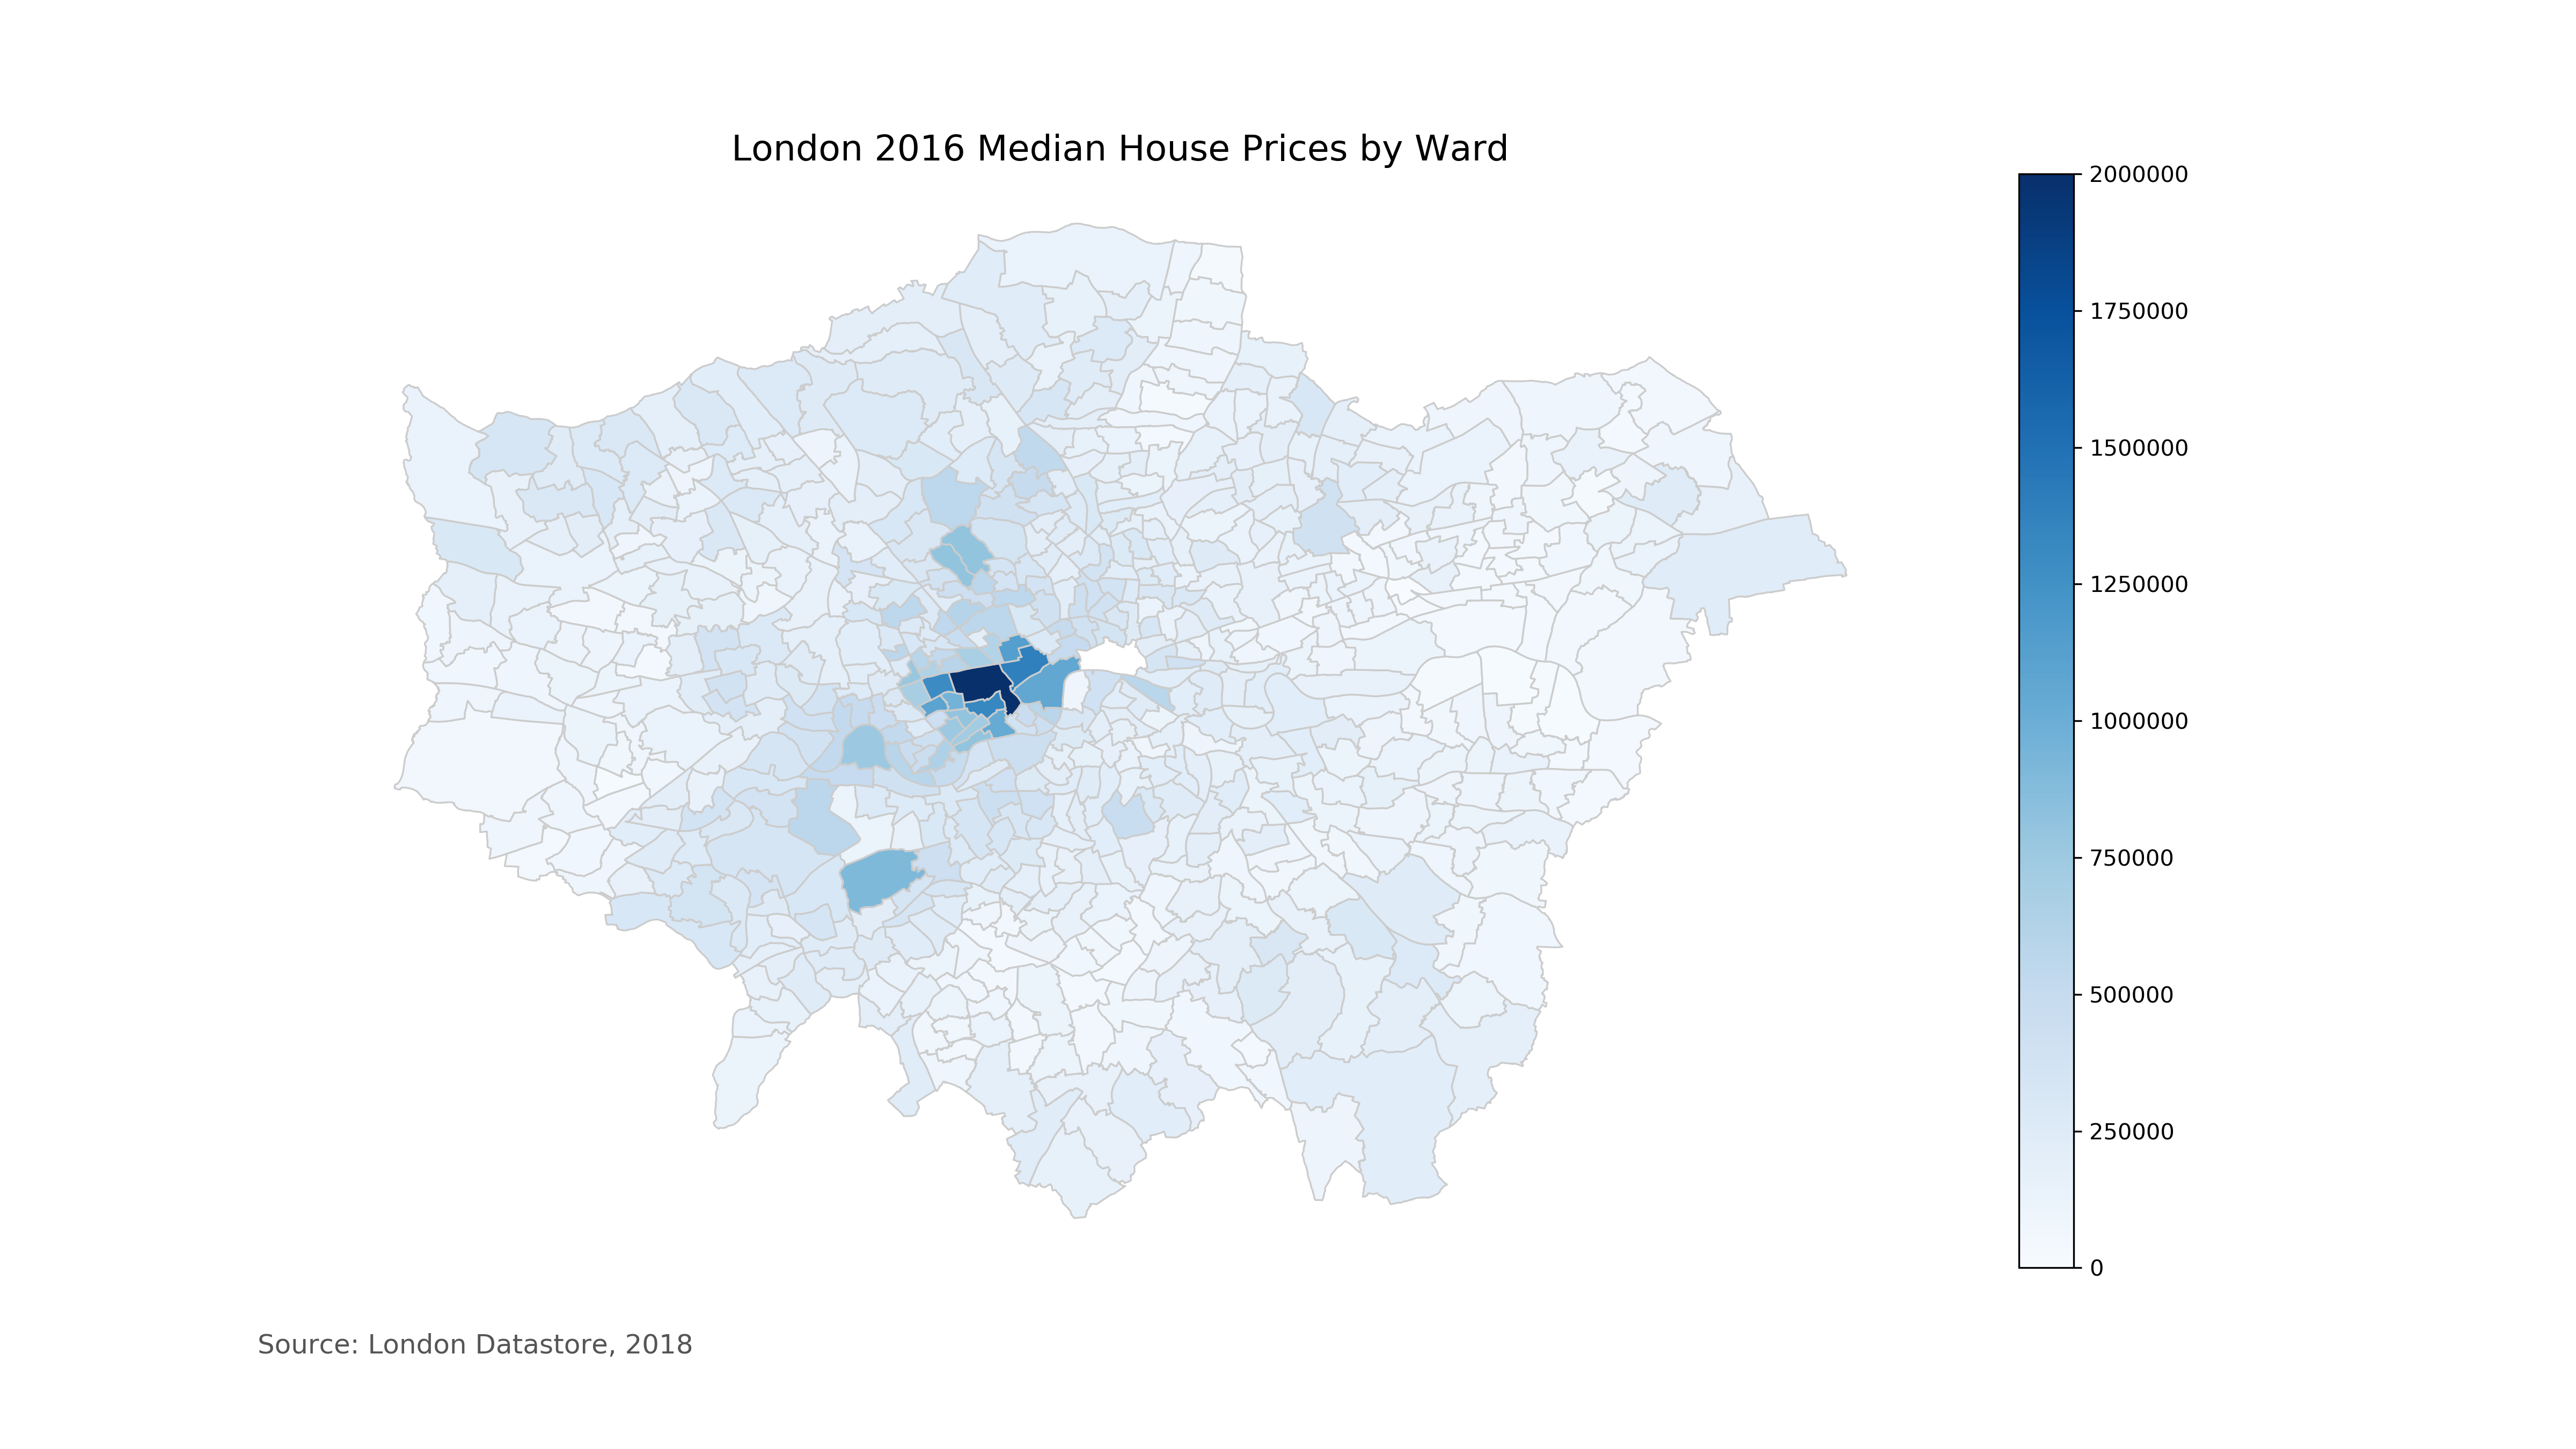
\includegraphics[scale=0.4]{figures/HPMedian}
\decoRule
\caption{Choropleth map showing median house prices for each ward in London (based on values at the end of 2017).}
\end{figure}

The choropleth map would suggest a high number of wards fall at the lower end of the range of median house prices with a small number with significantly high prices. From the pairwise plot below, the shape of the histogram of median house prices by ward would suggest that a power law may best describe the distribution.

\begin{equation}
p(x) = x^{-4.314410441437625}
\label{eqn:Einstein}
\end{equation}

For the indices, the histograms show most of the six as being at least close to a normal distribution. This is less clear in the case of the Safety and Security and Community Vitality and Participation indices with Safety and Security showing a large number of high values and Community Vitality and Participation showing many low scores. This can be attributed to a small number of wards where crime is high and that wards in central London have much greater access to both cultural and social spaces as indicated on the maps below. In both cases, a power law may best describe these distributions.

\begin{figure}
\centering
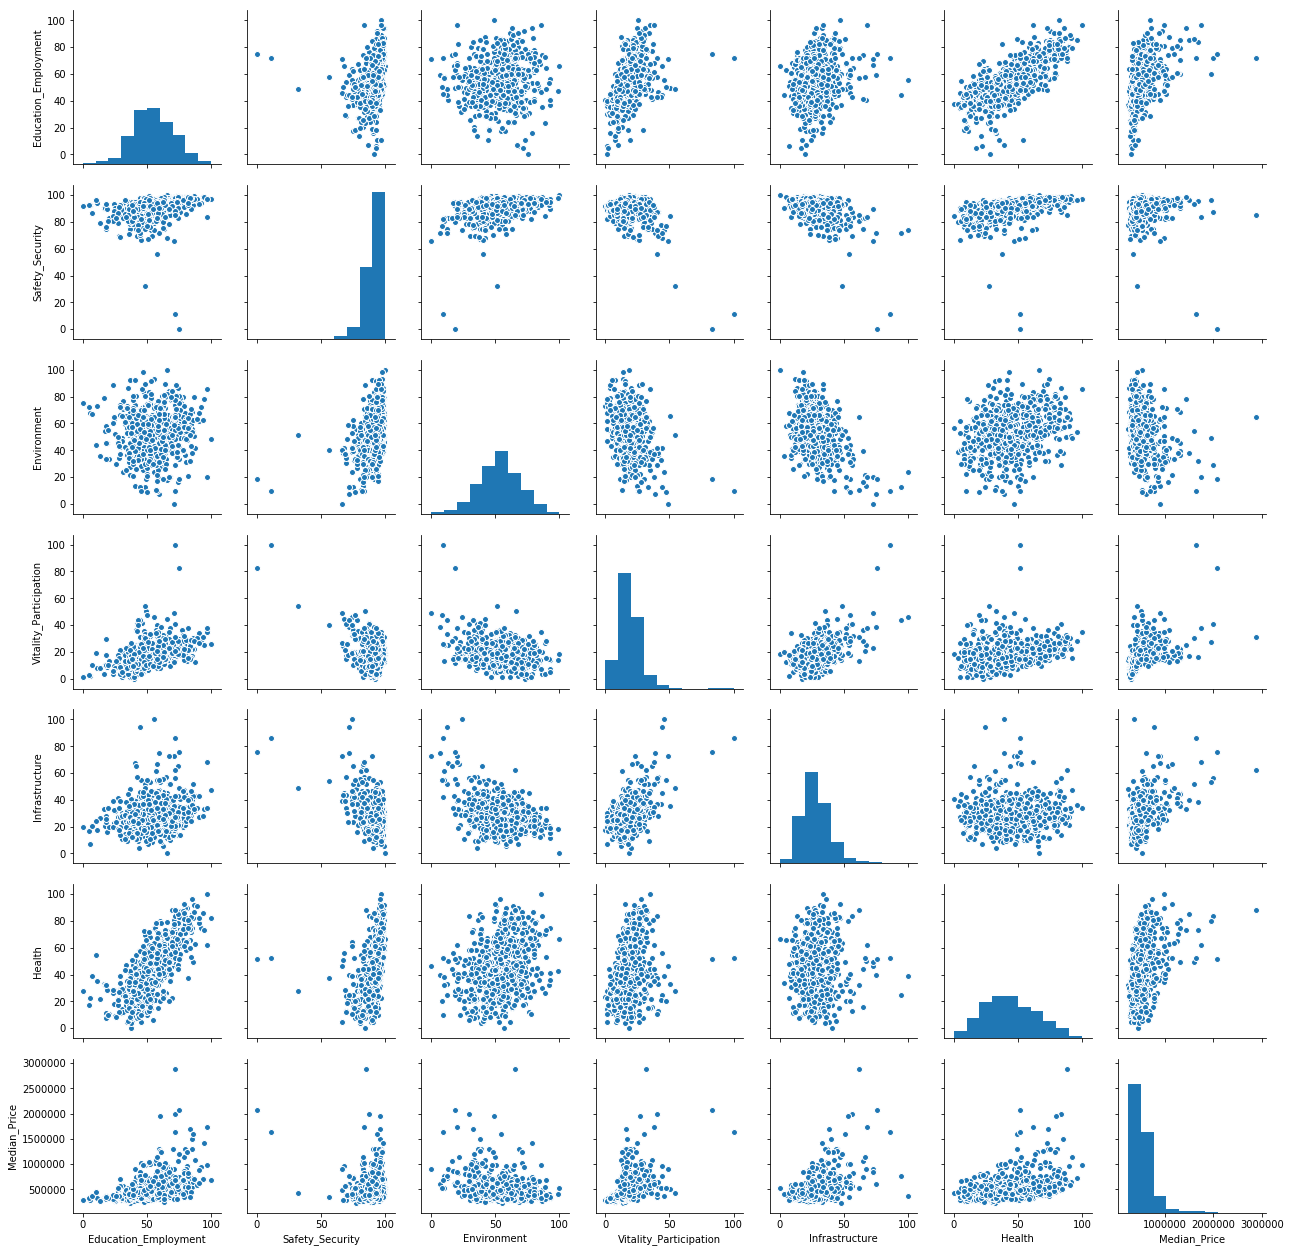
\includegraphics[scale=0.3]{figures/pairplot}
\decoRule
\caption{Pair-wise plot of the six well-being indices London median house prices with histograms showing the distribution of each index and house prices.}
\end{figure}

This is less clear in the case of the Safety and Security and Community Vitality and Participation indices with Safety and Security showing a large number of high values and Community Vitality and Participation showing many low scores. This can be attributed to a small number of wards where crime is high and that wards in central London have much greater access to both cultural and social spaces as indicated on the maps below. In both cases, a power law may best describe these distributions.

? CORRELATIONS ?

%----------------------------------------------------------------------------------------
%	SECTION 4
%----------------------------------------------------------------------------------------

\section{London house prices as a classification problem}
The choropleth map below shows a different picture of London house prices being based on quintiles rather than monetary values, here the fifth quintile covers a larger range of values than the other quintiles due to the extremely expensive areas such as Knightsbridge and Belgravia where the median house price reaches over £2.8 million, 10 times as much as North End ward in Bexley.

\begin{figure}
\centering
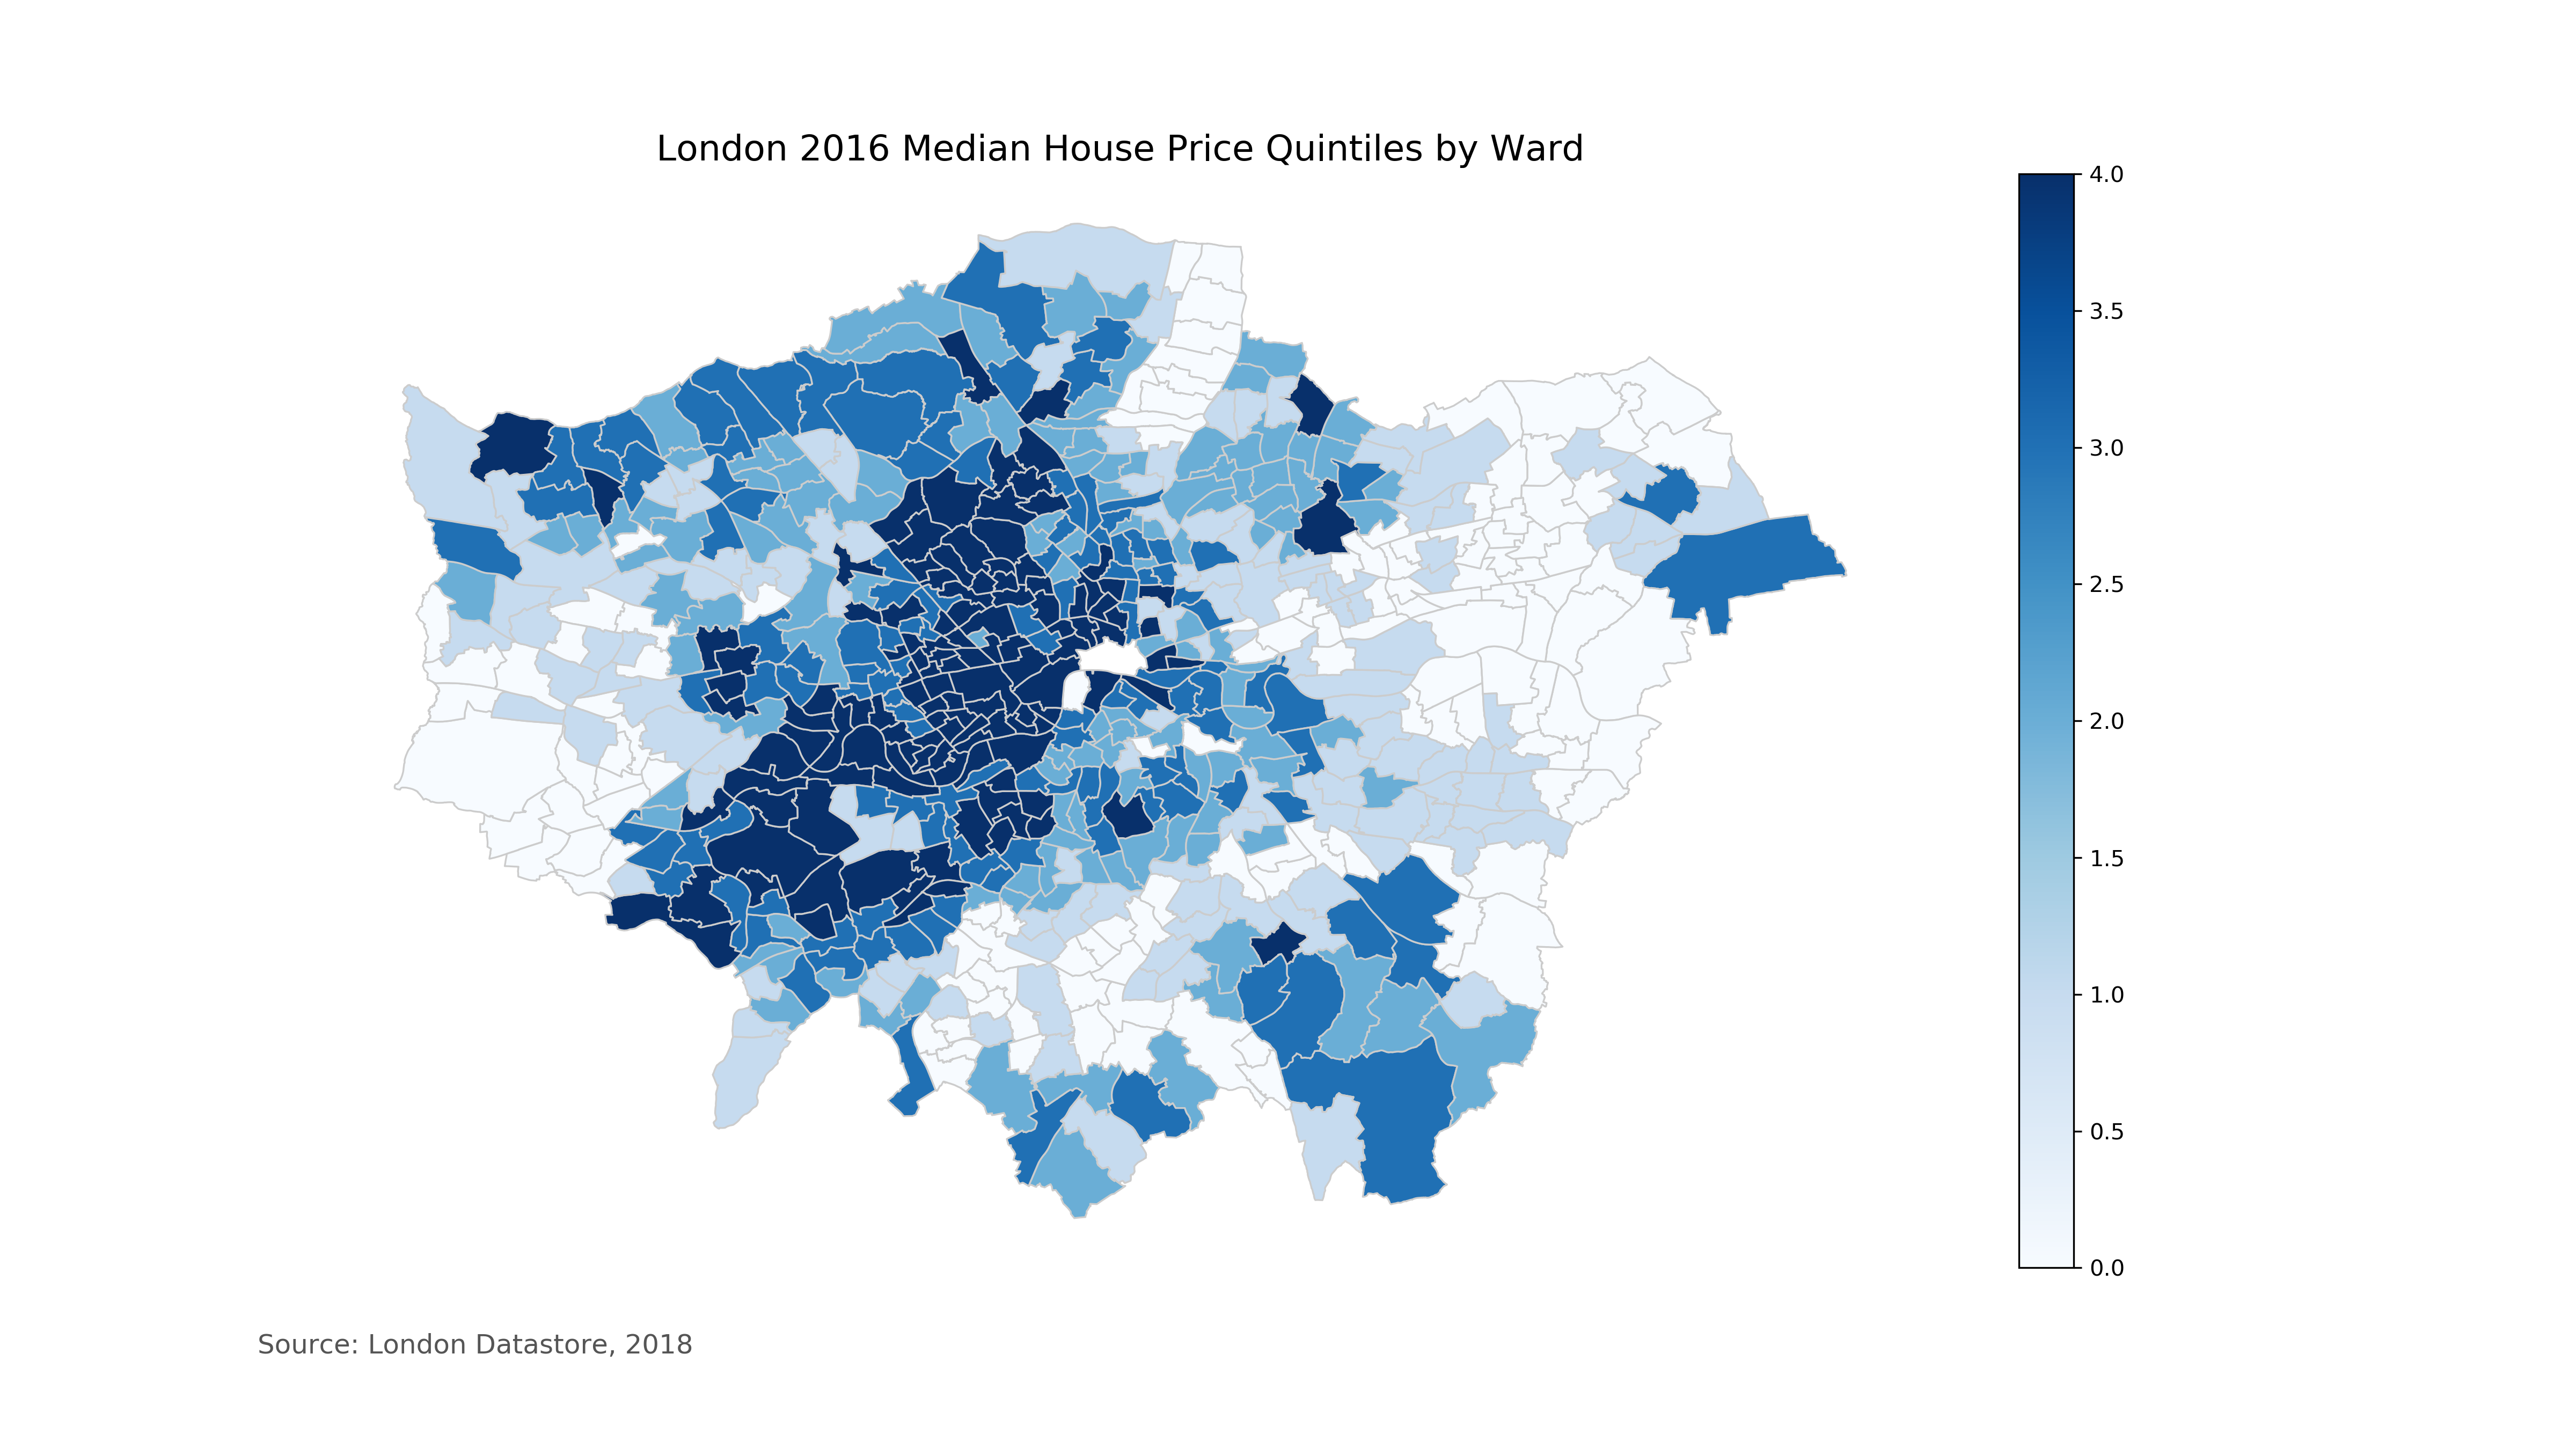
\includegraphics[scale=0.4]{figures/HPQuintile}
\decoRule
\caption{Choropleth map showing median house prices by for each ward in London by quintile (based on values at the end of 2017).}
\end{figure}

? BOXPLOT WITH QUINTILES ?

For the classification problem the aim was to try to find a model that has both a good fit and high interpretability. However, models that often have high accuracy but low interpretability such as neural networks were also used to both discover and validate the best classification model for the problem.

\begin{figure}
\centering
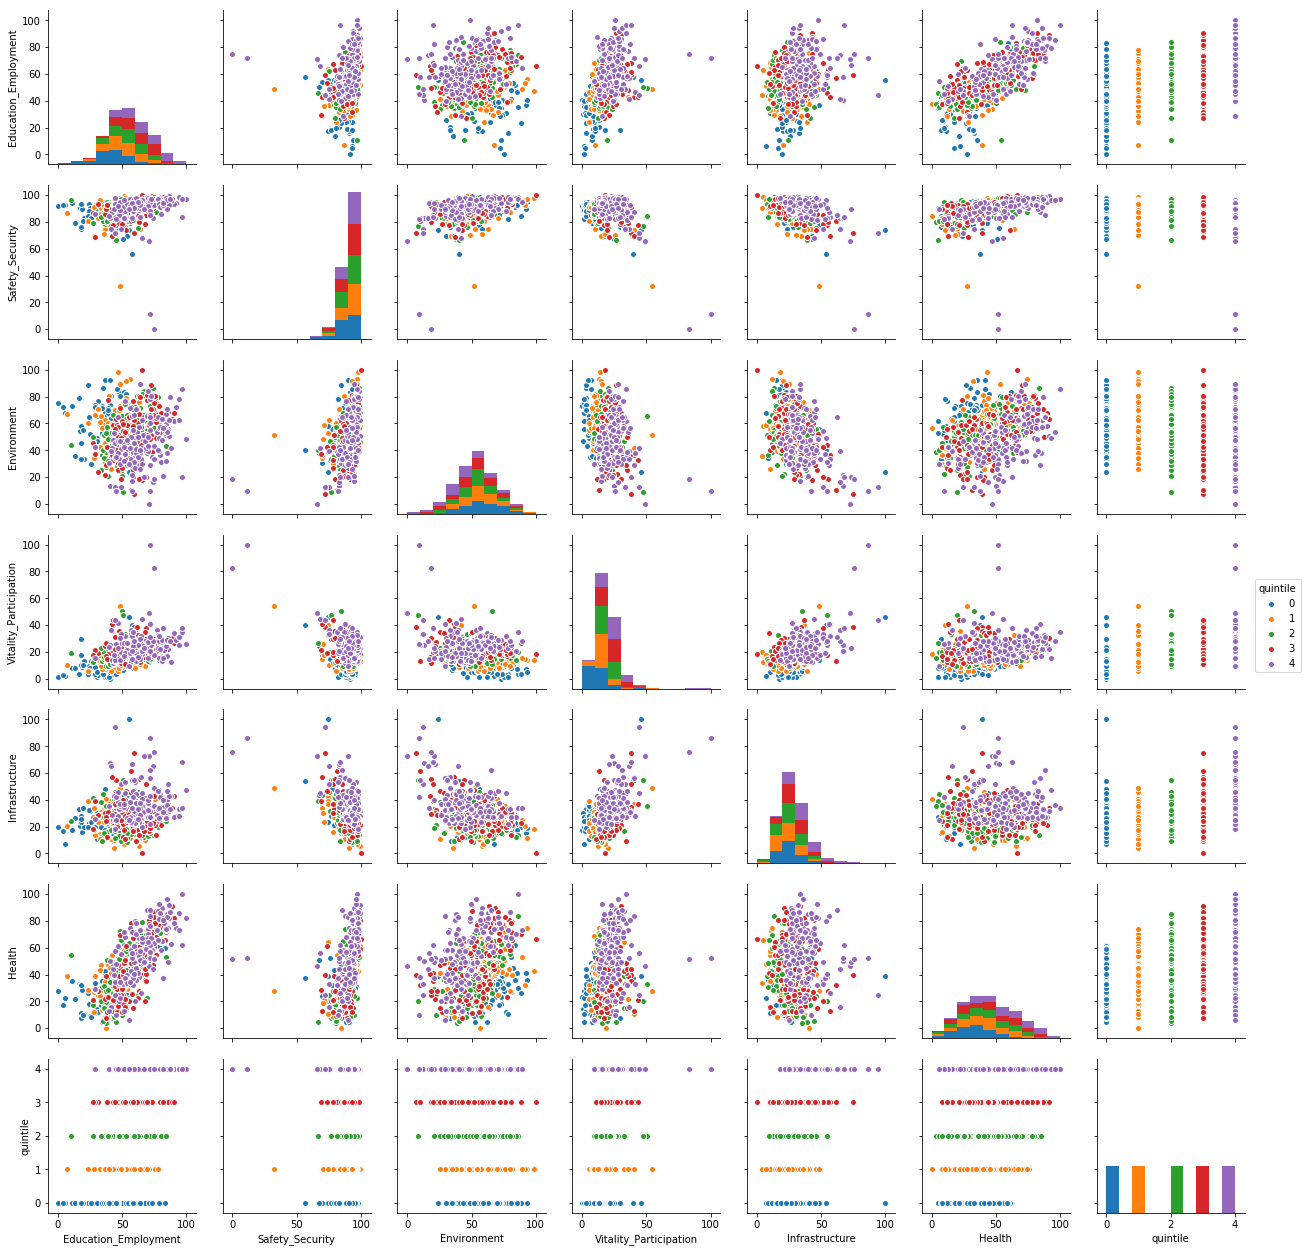
\includegraphics[scale=0.3]{figures/pairplot_quintile}
\decoRule
\caption{Pair-wise plot of the six well-being indices London median house prices with histograms showing the distribution of each index and house prices. Points are coloured on the basis of the quintile of the median house price within London ward.}
\end{figure}

By using the pair-wise plot and colouring the points by quintile, it is clear that there is no clear separation of quintile for any of the indices with a more gradual movement from first to fifth quintile for most domains. Environment and Saftey and Security have an almost inverse relationship with the quintiles. Because the majority of the high-priced wards are centrally located, this may relate to a lack of greenspace and higher polution centrally as well as providing high-value targets for crime. 